% Preamble from AmNat template
\documentclass[11pt]{article}
\usepackage[sc]{mathpazo} %Like Palatino with extensive math support
\usepackage{fullpage}
\usepackage[authoryear,sectionbib,sort]{natbib}
\linespread{1.7}
\usepackage[utf8]{inputenc}
\usepackage{lineno}
\usepackage{titlesec}
\titleformat{\section}[block]{\Large\bfseries\filcenter}{\thesection}{1em}{}
\titleformat{\subsection}[block]{\Large\itshape\filcenter}{\thesubsection}{1em}{}
\titleformat{\subsubsection}[block]{\large\itshape}{\thesubsubsection}{1em}{}
\titleformat{\paragraph}[runin]{\itshape}{\theparagraph}{1em}{}[. ]\renewcommand{\refname}{Literature Cited}

% other elements not in template
\usepackage[dvipsnames]{xcolor}
\usepackage[nointegrals]{wasysym}
\usepackage{gensymb}
\newcommand{\tom}[1]{{\textit{\color{WildStrawberry}{[#1]}}}}
\def\code#1{\texttt{#1}}
\usepackage{amsmath}
\usepackage{bm}
\usepackage{hyperref}
\usepackage{longtable}
\newcommand{\sym}[1]{\rlap{#1}}
\usepackage{tabularx}
\newcolumntype{L}[1]{>{\raggedright\arraybackslash}p{#1}}
\newcolumntype{C}[1]{>{\centering\arraybackslash}p{#1}}
\newcolumntype{R}[1]{>{\raggedleft\arraybackslash}p{#1}}
\usepackage{relsize}
\usepackage{booktabs}
\usepackage{graphicx}
\usepackage{float}
\usepackage{printlen}
\usepackage[section]{placeins}
\usepackage{afterpage}
\usepackage{caption}
\DeclareCaptionFormat{myformat}{#1#2#3\hrulefill}
\captionsetup[figure]{format=myformat}
%%%%%%%%%%%%%%%%%%%%%
% Line numbering
%%%%%%%%%%%%%%%%%%%%%
%\usepackage{lineno}
% Please use line numbering with your initial submission and
% subsequent revisions. After acceptance, please turn line numbering
% off by adding percent signs to the lines %\usepackage{lineno} and
% to %\linenumbers{} and %\modulolinenumbers[3] below.

\title{Demography-dispersal trait correlations modify the eco-evolutionary dynamics of range expansion}

% This version of the LaTeX template was last updated on
% January 11, 2018.

%%%%%%%%%%%%%%%%%%%%%
% Authorship
%%%%%%%%%%%%%%%%%%%%%
% Please remove authorship information while your paper is under review,
% unless you wish to waive your anonymity under double-blind review. You
% will need to add this information back in to your final files after
% acceptance.

\author{Brad M. Ochocki \\
Julia B. Saltz \\
Tom E.X. Miller$^{\ast}$}

\date{}

\begin{document}

\maketitle

\noindent{} Department of BioSciences, Program in Ecology and Evolutionary Biology, Rice University, Houston, TX 77005

\noindent{} $\ast$ Corresponding author; e-mail: tom.miller@rice.edu.

\bigskip

\textit{Manuscript elements}: Figure 1, Figure 2, Figure 3 (to print in color), Figure 4 (to print in color), Table 1, Online Appendix A (including Table A1), Online Appendix B (including Figures B1 and B2).

\bigskip

\textit{Keywords}: spatial selection, life-history evolution, trait correlations, G-matrix, biological invasion.

\bigskip

\textit{Manuscript type}: Article.

\bigskip

\noindent{\footnotesize Prepared using the suggested \LaTeX{} template for \textit{Am.\ Nat.}}

\linenumbers{}
\modulolinenumbers[3]

\newpage{}

% Abstract -------------
\section*{Abstract\footnote{\tom{7 words too long}}}
Spreading populations are subject to evolutionary processes acting on dispersal and reproduction that can increase the speed and variability of invasion. It is typically assumed that dispersal and demography traits evolve independently but abundant evidence points to correlations between them that may be positive or negative, genetic or environmental. We sought to understand how demography-dispersal correlations modify the eco-evolutionary dynamics of range expansion. We first explored this question with the beetle \textit{Callosobruchus maculatus}, a laboratory model in which evolutionary acceleration of invasion has been demonstrated. We then built a simulation model to explore the role of trait correlations in this system and more generally. We found that positive correlations amplify the positive influence of evolution on speed and variability, while negative correlations (such as we found empirically) constrain that influence. Strong negative genetic correlations can even cause evolution to decelerate invasion. Heritable and environmental correlations had similar effects on some measures of invasion but different effects on others. Model results allowed us to retrospectively explain invasion dynamics and trait evolution in \textit{C. maculatus}, and may similarly aid in the interpretation of other field and laboratory studies. Non-independence of demography and dispersal is an important consideration for understanding and predicting outcomes of biological invasion and climate change migration.

\newpage{}

% Introduction -------------
\section*{Introduction}
Understanding the factors that govern the rate of spatial expansion is a long-standing problem in population biology and takes on urgency in the context of two key dimensions of contemporary global change: range expansion by invasive species and climate change migration by native species.
Classic ecological theory tells us that the dynamics of range expansion are driven by the combined forces of local birth/death processes (`demography') and individual movement (`dispersal') \citep{skellam_random_1951,okubo_diffusion_1980,kot_discrete-time_1986,kot_dispersal_1996}.
Recently, ecologists have begun to examine the consequences of individual variation, especially heritable variation, in demography and dispersal traits and how eco-evolutionary feedbacks can modify the dynamics of range expansion.

Individuals that vary in dispersal ability are expected to become sorted along an expanding population front \citep{shine_evolutionary_2011}.
Spatial sorting generates an over-representation of highly dispersive phenotypes at the invasion vanguard.
If dispersal is heritable, non-random mating among highly dispersive individuals may lead to rapid evolution of increased dispersal ability at the leading edge.
Furthermore, if density-dependent demography generates a fitness advantage at the low-density invasion front, highly dispersive alleles may be favored by `spatial selection' \citep{phillips_life-history_2010, perkins_evolution_2013}.
Increased fitness in the vanguard can also result in natural selection for increased low-density reproductive rates (`\textit{r}-selection’) \citep{phillips_life-history_2010}.
Because, under a wide range of conditions, invasion speed is determined by dispersal and low-density reproductive rate, the combined action of these evolutionary processes is expected increase the speed of invasions \citep{phillips_evolutionary_2015}. A surge of recent experimental work supports this theoretical prediction \citep{williams_rapid_2016, ochocki_rapid_2017, weiss-lehman_rapid_2017,van2018kin}.
Several studies also show more variation in speed -- how far the invasion spreads over time -- than would be expected in the absence of evolution \citep{phillips_evolutionary_2015, ochocki_rapid_2017, weiss-lehman_rapid_2017}.
Increased variability is likely due to the stochastic fixation of alleles at the leading edge, which is a consequence of the serial founder events that characterize invasive spread -- a spatial analogue of genetic drift called `gene surfing' \citep{edmonds_mutations_2004,klopfstein_fate_2006,excoffier_surfing_2008,peischl_expansion_2015,phillips_evolutionary_2015, ochocki_rapid_2017, weiss-lehman_rapid_2017}.

Most theoretical models of the eco-evolutionary dynamics of range expansion assume that dispersal and low-density reproductive rate (hereafter `fertility') evolve independently.
If, however, these traits are genetically correlated then it impossible to predict the outcome of selection without knowing both the magnitude and sign of the correlation \citep{lande_measurement_1983,chenoweth2010contribution}.
Quantitative genetics offers a convenient framework to explore sources of (co)variation in ecologically important traits.
In the simplest case, total phenotypic variation in a single quantitative trait can be partitioned into two types of variance: additive genetic variance (the variance that can be explained by the inheritance of alleles) and environmental variance (any residual, non-heritable variance caused by extrinsic factors) \citep{lynch_genetics_1998,kruuk_estimating_2004,wilson_ecologists_2010}.
This framework can be extended to account for multiple traits and the correlations between them.
Genetic correlations may arise through pleiotropy (a subset of genes influencing multiple traits) and/or physical linkage (association of alleles on chromosomes) \citep{roff_evolutionary_1997} while environmental correlations arise from plastic responses to the environment that are non-independent across traits.
There are, then, many ways for dispersal and fertility to interact via trait correlations; the correlations can be positive or negative, and can be due to genetic effects, environmental effects, or both.

Due to the energetic cost of dispersal, it is often assumed that negative correlations in the form of trade-offs between dispersal and life-history traits should be important drivers of invasion dynamics \citep{hanski_dispersal-related_2006,chuang_expanding_2016}.
However, it it is not clear that we should expect to see such bivariate trade-offs in nature \citep{saltz_trait_2017}, or even that trade-offs should necessarily be associated with negative genetic correlations \citep{houle_genetic_1991}.
In the Glanville fritillary butterfly (\textit{Melitaea cinxia}), variation tightly linked to a single gene (\textit{Pgi}) generates a positive genetic correlation between dispersal propensity and clutch size \citep{hanski_dispersal-related_2006,bonte_dispersal_2012}.
Conversely, speckled wood butterflies (\textit{Pararge aegeria}) at range margins demonstrate a heritable negative correlation between dispersal propensity and clutch size \citep{hughes_evolutionary_2003}, while the damselfly \textit{Coenagrion scitulum} exhibits no genetic correlation between dispersal and clutch size \citep{therry_higher_2014}.
Environmental correlations, on the other hand, may arise through any number of extrinsic, non-heritable factors that generate plastic phenotypic responses.
Female blue tits (\textit{Parus caeruleus}) show a positive environmental correlation between dispersal and future fertility that is related to current brood size: females that were experimentally assigned to rear small broods in one year dispersed farther and had increased fertility in the following year relative to females assigned large broods \citep{nur_consequences_1988}.
Negative environmental correlations between dispersal and fertility have been demonstrated in the green-veined white butterfly (\textit{Pieris napi}), where individuals exposed to a controlled temperature/photoperiod regime that mimicked summertime conditions had higher dispersal and lower fertility than individuals exposed to a springtime regime \citep{karlsson_seasonal_2008}.
Indeed, widespread evidence for dispersal `syndromes' -- the covariation of dispersal with other life history and behavioral traits within \citep{clobert2009informed} or between \citep{comte2018evidence,stevens2014comparative} species -- suggests that the classical assumption of demography and dispersal rates as independent parameters may break down for eco-evolutionary models that incorporate trait heterogeneity.
How, then, should we expect the magnitude and sign of demography-dispersal covariance to alter predictions about range expansion?

Only two previous studies, to our knowledge, have explored eco-evolutionary dynamics of spread under trade-offs (negative correlation) between life history traits, focusing on the trade-off axis of \textit{r}/\textit{K} selection \citep{burton_trade-offs_2010,perkins_after_2016}.
These studies suggest that, for populations invading empty space, traits that promote fertility and dispersal should be maintained at the invasion front at the expense of competitive ability \citep{burton_trade-offs_2010,perkins_after_2016}.
However, because they imposed a particular type of trade-off, these studies do not reveal how variation in the sign and magnitude of genetic and/or environmental trait correlations modify spread dynamics.
Furthermore, although there is an expectation that evolutionary processes can make invasions more variable \citep{phillips_evolutionary_2015,ochocki_rapid_2017,weiss-lehman_rapid_2017}, it is not clear how genetic and/or environmental correlations interact with other evolutionary processes to influence variability in invasion outcomes.
Understanding the factors that drive invasion variability is essential for making useful predictions about the range of possible trajectories for spreading populations.
%The hunt for sources of invasion variability is thus an active area of research \citep{melbourne_highly_2009,wagner_genetic_2016,miller_sex_2013}. 
%\tom{[I have the hypothesis that environmental correlations should increase variance, but only in variable abiotic environments. If the spatial environment is constant then there is no way for this correlation to manifest. If the spatial environment is itself variable then there should be wider fluctuations in trait values at the front (if E correlation is positive). Worth testing/adding? How?]}-- add to discussion
%I am experimenting with cutting these hypotheses, for the sake of both length and thunder
%We hypothesize that negative genetic correlation between dispersal and fertility may constrain evolutionary acceleration of spread, relative to invasions with independent trait evolution, because high-dispersal / high-fertility phenotypes may be inaccessible to selection. %\tom{[It is not clear in the case of negative correlation whether dispersal or fertility would increase at front, if both cannot. Might be worth adding.]}
%Alternatively, positive correlation may align the direction of selection with the main axis of phenotypic covariation, causing greater evolutionary responses than would be expected for uncorrelated traits.
%We further hypothesize that environmental correlations, positive or negative, should have little impact on evolutionary dynamics of invasion; since environmental correlations modify traits in a way that is not heritable, they may contribute little more than noise at the invasion front.

In this study, we used a combination of laboratory experiments, classical quantitative genetics, and individual-based models to explore how demography-dispersal trait correlations, arising from genetics and/or environment, influence trait evolution during range expansion and the ecological dynamics of spread.
We explored this question first in a specific empirical setting, building on a model system for the evolutionary acceleration of range expansion, and then more generally.
In a previous study, we showed that rapid evolution accelerated the expansion of bean beetles (\textit{Callosobruchus maculatus} (Chrysomelidae)) spreading through laboratory mesocosms and also elevated replicate-to-replicate variability in invasion speed \citep{ochocki_rapid_2017}.
Surprisingly, evolutionary acceleration was due entirely to rapid evolution of dispersal distance; there was no evidence that fertility evolved during range expansion despite predictions that it should \citep{ochocki_rapid_2017}.
Here, we quantified the architecture of these traits, including their genetic and environmental variances and covariances.
We then integrated experimental trait estimation with a spatially explicit, individual-based model that combines population genetics and density dynamics.
The model allowed us to retrospectively evaluate whether and how trait correlations contributed to the evolutionary effects on traits (increased dispersal, no change in fertility) and range expansion (increased mean and variance of invasion speed) that we observed in our previous study.
Next, we used the system-specific parameters as a starting point to ask, more generally across parameter space, how the full range of possible demography-dispersal trait correlations influence the eco-evolutionary dynamics of spread.
To our knowledge, our study is the first to connect trait covariance with  eco-evolutionary dynamics of invasion, a connection whose importance has been widely anticipated \citep{chuang_expanding_2016,phillips_life-history_2010,perkins_evolution_2013} but not previously demonstrated.

% Methods -------------
\section*{Materials and Methods}

We conducted this study in three parts.
First, we measured dispersal and density-dependent fertility from individuals with known pedigree.
This enabled us to infer the genetic and environmental variances and covariances (and thus correlations) between dispersal and fertility using hierarchical Bayesian estimation of a quantitative genetics model.
Second, we used estimates from this statistical model to parameterize a stochastic simulation of bean beetle range expansion.
The model allowed us to generate system-specific predictions for evolved trait changes and spread dynamics.
Lastly, we varied the genetic and environmental (co)variances of dispersal and fertility, beyond the particular values of the beetle system, to more generally evaluate how trait correlations influence invasion dynamics.

\subsection*{Bean beetle experiment}

\subsubsection*{Study system}

The bean beetle \textit{Callosobruchus maculatus} is a stored-grain pest that feeds on legumes, spending its entire developmental life inside a single bean \citep{fujii_behavioral_1990}.
Adult beetles, which requires neither food nor water, emerge after ca. 28 days of development.
Adults live ca. 10 days, during which they disperse, mate, and reproduce.
The short generation time and convenient rearing conditions make this species is a popular model system in population biology, including previous studies of life-history traits, population dynamics, and range expansion \citep{bellows_analytical_1982,fujii_behavioral_1990,miller_confronting_2011,miller_sex_2013,wagner_genetic_2016,ochocki_rapid_2017}.

Laboratory populations of \textit{C. maculatus} are typically highly inbred, often for dozens or hundreds of generations.
We created a genetically diverse population that was founded with 54 beetles (\female:\mars $\approx$ 1:1) haphazardly chosen from each of 18 laboratory lines (960 beetles in total), each line having been originally isolated from different parts of the species’ global distribution \citep{downey_comparative_2015}.
This was the same genetic make-up of the populations used in our previous range expansion experiments \citep{ochocki_rapid_2017}.
Individuals in this mixed population interbred in a resource-unlimited environment for seven generations before the start of the experiment, to allow for sufficient genetic mixing and to reduce linkage disequilibrium \citep{roughgarden_theory_1979,ochocki_rapid_2017}.
Beetles were maintained in a climate-controlled growth chamber on a 16:8 photoperiod at 28$^{\circ}$C throughout the experiment.
The beetles used in this experiment were reared on black-eyed peas (\textit{Vigna unguiculata} (Fabaceae)). %Beetles from different laboratory lines readily interbreed and produce fertile offspring \citep{fox_complex_2004,fox_genetic_2004,ochocki_rapid_2017}.

\subsubsection*{Trait measurement}
\paragraph{Dispersal}
We used a nested full-sib/half-sib breeding design to measure genetic and environmental variances and covariances in our laboratory-reared populations of \textit{C. maculatus}.
This design is appropriate because it allows the estimation of these variances from a single generation of trait measurement and does not require information on the parental genotypes or phenotypes \citep{falconer_introduction_1996,conner_primer_2004,wilson_ecologists_2010}.
We created half-sib families by mating a single sire to three virgin dams, and replicated this process 50 times to get 150 unique full-sib families, each nested within one of 50 half-sib families.
After a 48-hour mating period, each dam was transferred to an individual Petri dish for oviposition.
Petri dishes contained 50g black-eyed peas, essentially unlimited resources for a single female, and dams were permitted to oviposit \textit{ad libitum} until senescence.
After 28 days of development, we measured dispersal and density-dependent fertility in the adult offspring.

Within 48 hours of eclosion, we measured dispersal ability by allowing beetles to disperse for two hours across one-dimensional arrays of 60mm Petri dish `patches'.
Each patch in these arrays was interconnected by 1/8" plastic tubing and contained seven black-eyed peas, the same dispersal environment as in our range expansion experiments \citep{ochocki_rapid_2017}.
Dispersal trials began with 16 full-siblings (8 females and 8 males) in a starting patch, with a sufficient number of patches to the left and right so that beetles could disperse in either direction without encountering the edge of the environment.
We chose to use 16 beetles because that was the largest number of individuals that we could reliably obtain from our full-sibling families while maintaining a 1:1 sex ratio among the dispersing individuals.
After two hours of dispersal, we recorded the number of patches that each beetle dispersed, which allowed us to estimate a dispersal kernel for each full-sibling family.

\paragraph{Fertility}
After dispersal, we gathered female beetles and transfered each of them to an isolated Petri dish where they could oviposit; after 28 days we counted the number of offspring that emerged to estimate a fertility for each female.
While our main focus was low-density fertility in leading-edge environments, we additionally quantified density dependence in fertility so that our simulations could include realistic population dynamics behind the advancing front.
To induce density-dependence in fertility, each oviposition dish contained a resource density of either 1, 3, 5, or 10 black-eyed peas, and a non-sibling male beetle.
Given the opportunity, females will attempt to distribute their eggs approximately uniformly among available beans \citep{fujii_behavioral_1990} so that the number of eggs per bean is inversely proportional to the number of beans available.
Larval competition within a bean has a strong negative effect on larval survival to adulthood, so that any larva's survival probability decreases with the number of eggs per bean \citep{giga_intraspecific_1991}.
It is therefore possible to vary the strength of larval competition that offspring experience simply by varying the number of beans available to females for oviposition.
Thus, dishes containing one black-eyed pea were expected to yield high egg densities, resulting in high-competition larval environments; dishes containing 10 black-eyed peas were expected to yeild low egg densities, resulting in low-competition larval environments.
Post-dispersal females were haphazardly assigned to one of the four oviposition densities.
Due to the relatively low number of female dispersers in each full-sibling family, we opportunistically supplemented fertility trials with full-sibling females that were not included in the dispersal trial.
We attempted to replicate each bean density at least three times per full-sib family; we made note of fertility trials using un-dispersed females, and preliminary analyses did not reveal any differences in fertility between dispersed and un-dispersed individuals.

Since the density-dependent competition described here is among full siblings, it is important to consider whether competition among full siblings might be different than competition among unrelated individuals.
Conveniently, experimental evidence shows that the strength of competition among developing larvae of \textit{C. maculatus} does not vary with relatedness \citep{smallegange_local_2008}.
Thus, changes in fertility in response to changing resource availability under this design likely reflect true measures of intraspecific competitive ability, and are likely not influenced by reduced competition due to kinship.


\subsubsection*{Statistical analysis}
\paragraph{Overview}
We used the animal model to estimate genetic and environmental variances and covariances of dispersal and demography traits \citep{lynch_genetics_1998,kruuk_estimating_2004,wilson_ecologists_2010}.
The animal model is hierarchical linear mixed model that partitions genetic variance in quantitative traits based on associations between kinship and trait values of offspring, even if trait values of parents are not known (as in our study).
Because dispersal and fertility were measured as counts (patches moved and number of offspring, respectively) we used a generalization of the animal model for non-Gaussian traits \citep{de2016general}.
This distinction is important because, in the generalized animal model, genetic variation in traits manifests at two scales: the scale of the observations and a `latent' scale that corresponds more directly to the trait values expected due to kinship but that can only be studied through random realizations \citep{de2016general}.
As we describe in the next sections, we focus throughout on genetic variace, covariance, and heritability of dispersal and demography traits on their latent scales.

While the animal model framework is able to accommodate additional random effects associated with maternal environmental (i.e., maternal effects), our model failed to converge when we attempted this, indicating that our data were not sufficient to estimate maternal effects in addition to other sources of variance and covariance.
Any maternal effects are therefore implicitly incorporated into kinship, which may positively bias estimates of additive genetic variance and narrow-sense heritability.
Also, males and females in \textit{C. maculatus} are known to differ in dispersal \citep{miller_sex_2013,ochocki_rapid_2017}.
Since we could only measure density-dependent fertility in females, we focused our analysis exclusively on data collected from females and the the simulation model that follows is correspondingly female-dominant.

\paragraph{Dispersal}
Previous studies estimating \textit{C. maculatus} dispersal kernels have found negative binomial or Poisson Inverse Gaussian kernels to provide the best fit to dispersal data \citep{miller_sex_2013,wagner_genetic_2016,ochocki_rapid_2017}.
While this was also the case in the present study when data were aggregated across families, a Poisson kernel provided the best fit to family-level dispersal data.
This is likely due to the fact that heterogeneity in the mean among families generates an aggregate response that is negative-binomially distributed.
We thus modeled the dispersal distance $d$ of individual $i$ from sire $j$ and dam $k$ as:
%
\begin{equation}\label{corr:dispersal_random}
  d_{ijk} \sim \mathit{Poisson}(\lambda_{ijk})
\end{equation}
%
where $\lambda_{ijk}$ is the mean and variance of the Poisson distribution.
The expected value for dispersal distance is defined by a linear model that includes a grand mean ($\mu^{d}$) and accounts for parentage ($a^{d}_{jk}$) and residual deviation of observation $i$ ($e^{d}_i$):
%
\begin{equation} \label{corr:dispersal_linmod}
  log(\lambda_{ijk}) = \mu^{d} + a^{d}_{jk} + e^{d}_{i}
\end{equation}
%
The genetic ($a^{d}_{jk}$) and environmental ($e^{d}_i$) random variables for dispersal distance are further defined below in relation to fertility.

\paragraph{Fertility}
\footnote{\tom{I think there is an error in these equations. Given the B-H model $N_{t+1}=\frac{rN_{t}}{1+bN_{t}}$, $b$ is derived as $\frac{r-1}{K}$. So that means Eq. \ref{corr:BevHoltFull} should be 
$\frac{N_{t+1}}{B} = \frac{r(\frac{N_{t}}{B})}{1 + \frac{r-1}{K}\frac{N_{t}}{B}}$
and corredponding changes to subsequent equations. 
I am not sure if this is an error just in the manuscript, or if there was also an error in the fitted model.
I tried checking Brad's code to see what he was actually fitting, but the stan code I found on github fits the B-H model with the original parameterization, not breaking out K. 
So I don't think this was the final version of the analysis. 
I will need Brad's help to figure this out.}}
Unlike dispersal, fertility was measured with respect to density.
We imposed density dependence by manipulating the resources available to an individual female rather than density \textit{per se}.
We analyzed the data using the framework of the Beverton-Holt model of population growth, modified so that population density is expressed as the ratio of females to beans:
%
\begin{equation}\label{corr:BevHoltFull}
  \frac{N_{t+1}}{B} = \frac{r(\frac{N_{t}}{B})}{1 + \frac{r}{K}\frac{N_{t}}{B}}
\end{equation}
%

Dividing both sides by $N_{t}/B$ and setting $N_{t}=1$ gives the expected offspring production of single females in variable bean environments:
%
\begin{equation}\label{corr:BevHoltPercap}
  \hat{N}_{t+1} = \frac{r}{1 + \frac{r}{KB}}
\end{equation}
%
Here, $B$ is the number of beans available, $r$ is low-density fertility, and $K$ is the carrying capacity per-bean (i.e., the number of beetles that one bean could support).
Our aim was to identify variation in $r$ that was attributable to pedigree and covariance with dispersal.
There is a well-documented covariance between statistical estimates of $r$ and $K$ in density-dependent population models \citep{hilborn_quantitative_1992}, and this prevented us from modeling both $r$ and $K$ as heritable traits.
Instead, we assume a fixed value of $K$ and allow $r$ to vary among individuals according to a quantitative genetic model of inheritance.

We treat the number of offspring produced by female $i$ from sire $j$ and dam $k$ ($N_{ijk}$) as a Poisson random variable, with the expected value given by Eq. \ref{corr:BevHoltPercap}.
% - Not sure it is worth showing this.
%
\begin{equation}\label{corr:Noff_ran}
  N_{ijk} \sim \mathit{Poisson}\Big(\frac{r_{ijk}} {1 + \frac{r_{ijk}}{KB_{ijk} }}\Big)
\end{equation}
%
As in Eq. \ref{corr:dispersal_linmod}, low-density fertility is described by a linear model that includes a grand mean ($\mu^{r}$) and accounts for parentage ($a^{r}_jk$) and residual deviation of observation $i$ ($e^{r}_i$):
%
\begin{equation} \label{corr:fert_linmod}
  log(r_{ijk}) = \mu^{r} + a^{r}_{jk} + e^{r}_{i}
\end{equation}
%

\paragraph{Linking dispersal and fertility}
Finally, to model genetic and environmental variances and covariances, we link the corresponding random deviates.
The vector $\bm{a}_{jk}$ contains the random deviates (also known as `breeding values') for dispersal ($a^{d}_{jk}$) and fertility ($a^{r}_{jk}$) associated with kinship and is distributed according to a multivariate normal distribution centered on the average of the breeding values for both parents (the `midparent value') with variance-covariance matrix $\bm{G}/2$:
%
\begin{gather} \label{corr:gen}
  \bm{a}_{jk} \sim \mathit{MVN} \Big( \frac{\bm{a}_{j} + \bm{a}_{k}}{2}, \frac{\bm{G}}{2} \Big) \\[10pt]
  \bm{G} =
  \begin{bmatrix}
    \begin{array}{ll}
      V_{G,d} &C_{G}   \\
      C_{G}   &V_{G,r} \\
    \end{array}
  \end{bmatrix}
\end{gather}
%
Here, $V_{G,d}$ and $V_{G,r}$ are the additive genetic variances in the `latent' trait values for dispersal and fertility and $C_{G}$ is the additive genetic covariance between between the latent trait values.
In Equation (\ref{corr:gen}), dividing $\bm{G}$ by $2$ accounts for the expected additive genetic variance among full siblings compared with the population as a whole \citep{roughgarden_theory_1979}

The environmental deviates -- individual-to-individual variation that is not explained by pedigree, also known as `overdispersion' \citep{de2016general} -- are treated similarly, where the vector $\bm{e}_{i}$ contains elements $e^{d}_{i}$ and $e^{r}_{i}$ from Eq. \ref{corr:dispersal_linmod} and Eq. \ref{corr:fert_linmod}, respectively, and is distributed as:
%
\begin{gather} \label{corr:env}
  \bm{e}_{i} \sim \mathit{MVN} (0, \bm{E}) \\[5pt]
  \bm{E} =
  \begin{bmatrix}
    \begin{array}{ll}
      V_{E,d} &C_{E}   \\
      C_{E}   &V_{E,r} \\
    \end{array}
  \end{bmatrix}
\end{gather}
%
In the bean beetle system, microsite variation in larval environment is a good candidate for the environmental variation $\bm{E}$, as host beans may vary in, for example, nutrient content, water content, geometry, age, etc.
For both covariances, genetic and environmental correlations were derived as $\rho = \frac{C}{\sqrt{V_{d}}\sqrt{V_{r}}}$. 
\footnote{\tom{I wrote this sentence, assuming this is where the heritabilities in Figure \ref{corr:posteriors} come from.
But I am actually not sure.
I would like to confirm with Brad.}}

Assuming that genetic and environmental effects are not correlated with each other, the total phenotypic variances and covariances in these traits can be described by a covariance matrix $\bm{P}$, which is simply $\bm{P} = \bm{G} + \bm{E}$.
Calculating $\bm{P}$ enables us to calculate the narrow-sense heritability of each trait, which reflects the proportion of variance in the phenotype (on the latent scale) attributable to additive genetic factors.
For dispersal,
%
\begin{equation}\label{corr:heritability}
  h^{2}_d = \frac{V_{G,d}}{V_{P,d}}
\end{equation}
%
and likewise for heritability of fertility ($h^{2}_r$).
All analyses in this section were performed in R 3.4.0 \citep{r_core_team_r:_2015} using \code{rstan} \citep{stan_development_team_rstan:_2015}.
Because models were fit in a Bayseian framework, we can quantify parameter uncertainty through their posterior distributions.
Code for these analyses may be found at \url{https://github.com/bochocki/correlatedtraits}.

\subsection*{Simulating invasions with correlated traits}
We simulated sexually-reproducing populations spreading across a one-dimensional landscape in discrete time and discrete space, based on our empirical estimates for \textit{C. maculatus} the system.
Although \textit{C. maculatus} has two sexes, we simulated hermaphroditic populations for tractability.
Each simulation began with 20 individuals in a single starting patch; we modeled each individual as expressing a dispersal and fertility phenotype following the statistical model defined above.
The additive genetic ($\bm{a}_{jk}$) and environmental deviates ($\bm{e}_i$) for each individual were drawn at random given covariance matrices $\bm{E}$ and $\bm{G}$, respectively (Eq. (\ref{corr:env}) and (\ref{corr:gen})).
The initial conditions of the simulation mimic a small founding population being introduced to an empty landscape from some genetically well-mixed source population. 
Complete details of the simulations are provided in Online Appendix A.
\footnote{\tom{I think we need to say something about whether or not our model allows correlations to evolve. I think yes, based on previous conversations with Brad, but I am not sure how to explain how or why this is so. Brad, can you add a sentence to this effect?}}

For analysis of the simulation output, we defined an invasion's extent in each generation as the location of the individual farthest to the right of the starting patch.
Since the duration of spread was fixed, the final extent is proportional to mean invasion speed (patches per generation), and this is how we frame the interpretation that follows.
%Because dispersal direction was unbiased, both the left- and right-moving wave fronts should exhibit similar dynamics, but we restricted our analysis to the right-moving fronts to avoid pseudo-replication.
To understand how trait variation and covariation altered simulated invasion outcomes, we focused on mean invasion extent after 20 generations and the coefficient of variation (CV) in extent as a measure of variability.
We quantified trait evolution in the simulations by comparing the genetically based quantitative trait values (population mean $\bm{\mu}$ plus breeding value $\bm{a}_{jk}$) between the value in the center patch in generation 0 and the value at the range-edge patch in generation 20.

We first ran the simulated invasions with parameter values estimated from the \textit{C. maculatus} laboratory experiments (Table \ref{corr:estimates}) to establish whether the model could generate invasion outcomes that were qualitatively consistent with our previous experimental work. % in terms of evolutionary effects on invasion speed and variability, as well as trait evolution underlying those effects.
We contrasted results against a `no evolution' scenario in which trait variation was not heritable ($h^{2}_d = h^{2}_r = 0$).
We did not attempt direct quantitative comparison between our previous experiment and present simulation because they differed in some known, important ways (e.g., for convenience, the simulations assumed hermaphroditism, and evolutionary effects were quantified with respect to a zero-heritability scenario rather than the spatial shuffle treatment of our previous experiment).
We generalized the \textit{C. maculatus}-specific results by exploring realistic variation in trait correlations, heritability, and phenotypic variance.
To test the role of variation in the sign and magnitude or trait correlations and contrast the effects of genetic vs. environmental correlations, we varied $\rho_{E}$ and $\rho_{G}$ factorially such that each correlation coefficient took a range of values (-0.9, -0.5, -0.1, 0, 0.1, 0.5, 0.9) in all combinations.
To further expand beyond the beetle system, we replicated the full range of trait correlations across variation in trait heritabilities and amount of total phenotypic variance. 
The complete parameter space of the simulations is described in Online Appendix A. 
We replicated each parameter combination 1000 times.

\renewcommand{\thetable}{\arabic{table}}
\setcounter{table}{0}

\newpage{}
\begin{table}[h]
\centering
\label{Estimates of key parameters from the beetle experiment}
\caption[Estimates of key parameters from the beetle experiment]{\textbf{Estimates of key parameters from the beetle experiment.} Parameter estimates are grouped by the demographic process that they correspond to: dispersal, fertility, or both. Percentages show parameter estimates in the 95\% credible interval and the median (50\%) parameter estimate.}\label{corr:estimates}\vspace{0.1in}
\begin{tabularx}{0.95\linewidth}{lXrrrrr}
\toprule
Parameter   & Description                               & Mean & SD   & 2.5\% & 50\% & 97.5\% \\ \midrule
$\mu_{d}$   & Mean dispersal phenotype (log(patches)) & 1.63 & 0.07 & 1.49   & 1.63 & 1.76   \\
$h^{2}_{d}$ & Dispersal heritability              & 0.55 & 0.17 & 0.22   & 0.54 & 0.91   \\
$V_{P,d}$   & Phenotypic variance in dispersal & 0.41 & 0.05 & 0.32   & 0.40 & 0.52   \\
$V_{G,d}$   & Additive genetic variance in dispersal & 0.23 & 0.09 & 0.08   & 0.21 & 0.45   \\
$V_{E,d}$   & Environmental variance in dispersal    & 0.18 & 0.06 & 0.04   & 0.18 & 0.30   \\ \midrule
$\mu_{r}$   & Mean fertility phenotype (log(offspring) & 2.74 & 0.07 & 2.61   & 2.74 & 2.87   \\
$h^{2}_{r}$ & Fertility heritability              & 0.17 & 0.07 & 0.05   & 0.16 & 0.31   \\
$V_{P,r}$   & Phenotypic variance in fertility & 0.35 & 0.02 & 0.30   & 0.35 & 0.40   \\
$V_{G,r}$   & Additive genetic variance in fertility & 0.06 & 0.03 & 0.02   & 0.06 & 0.12   \\
$V_{E,r}$   & Environmental variance in fertility    & 0.29 & 0.03 & 0.24   & 0.29 & 0.35   \\
$K$         & Carrying capacity per bean              & 3.82 & 2.59 & 3.34   & 3.81 & 4.36   \\ \midrule
$C_{P}$     & Total phenotypic covariance    &-0.08 & 0.02 &-0.13   &-0.08 &-0.03   \\
$C_{G}$     & Additive genetic covariance &-0.04 & 0.03 &-0.11   &-0.04 & 0.01   \\
$C_{E}$     & Environmental covariance   &-0.04 & 0.03 &-0.09   &-0.04 & 0.02   \\
$\rho_{G}$  & Additive genetic correlation  &-0.36 & 0.24 &-0.79   &-0.37 & 0.15   \\
$\rho_{E}$  & Environmental correlation     &-0.16 & 0.13 &-0.43   &-0.16 & 0.09   \\
\bottomrule
\end{tabularx}
\end{table}

% Results -------------
\section*{Results}

\subsection*{\textit{Architecture of \textup{C. maculatus} demography and dispersal traits}}
We found that demography and dispersal traits in \textit{C. maculatus} were linked through both additive genetic and environmental covariation.
There were similar amounts of total phenotypic variance in the latent traits corresponding to dispersal and fertility ($V_{P,d}$  = 0.40, $V_{P,r}$  = 0.35; Fig. \ref{corr:posteriors}, Table \ref{corr:estimates}
\footnote{\tom{Need to check with Brad about interpretation of phenotype values in this table. For example mean dispersal phenotype is 2.74. If I am correct that this is log offspring, then this equals 15.48 offspring, which is much less than the average in OandM 2017 Figure 4. However, maybe it is female offspring, which would make the value more reasonable.}}
), and both exhibited additive genetic variance, indicating that both traits are heritable from parents to offspring.
However, the  amount of genetic variance and therefore the proportion of heritable variation differed between the traits.
Dispersal had a median narrow-sense heritability ($h^{2}_{d}$) of 0.54 and the 95\% credible interval in the estimate spanned a wide range (0.22 to 0.91), suggesting moderate to strong inheritance of this trait.
The median narrow-sense heritability for fertility ($h^{2}_{r}$) was 0.17 and the 95\% credible interval spanned a lower and narrower range (0.05 to 0.31), reflecting less genetic variation in this trait compared to dispersal.

Correlations between dispersal and fertility were negative (Fig. \ref{corr:posteriors}), more so for the additive genetic effects (median $\rho_{G}$: -0.37) than the environmental effects (median $\rho_{E}$: -0.16).
While posterior distributions for both correlations included zero, the majority of both posterior densities were negative (Figure \ref{corr:posteriors}, center panel).
Given estimation uncertainty, as quantified by the Bayesian posterior probability distributions, the genetic correlation was \tom{$X$} times and the environmental correlation was \tom{$X$} times more likely to be negative than positive.
\footnote{\tom{[My thought here is that we should quantify how much of the posterior is negative vs positive, and this gives us a sense of confidence in the conclusion that correlations are negative.
As far as I am aware, I cannot do this myself because I don't have access to the posteriors.
So I think I will need Brad's help here. 
I think this is a simple but important addition, because from here on we assume that these negative correlations are real.]}}
%The estimated additive genetic correlation had a 95\% credible interval that was notably wider than the estimated environmental correlation ($\rho_{G}$: -0.79 to 0.15; $\rho_{E}$: -0.43 to 0.09).
%This occurs even though the credible intervals for the covariance estimates are similar to each other ($C_{G}$: -0.11 to 0.01; $C_{E}$: -0.09 to 0.02; Figure \ref{corr:posteriors}).
%This discrepancy is likely due to the relatively wide credible interval in the additive genetic variance in the dispersal trait ($V_{G,d}$: 0.08 to 0.45), which would necessarily result in a relatively wide credible interval in the additive genetic correlation.
%\tom{[I don't think this is super important but I actually do not follow this argument. I think part of my confusion is that I am not sure where the correlation estimates come from (comment above where you say they were ``calculated'').
%For related reasons, I think the covariances can be dropped from this figure, since they simply integrate the variances and correlations.]}

\begin{figure}[h!]
\centering
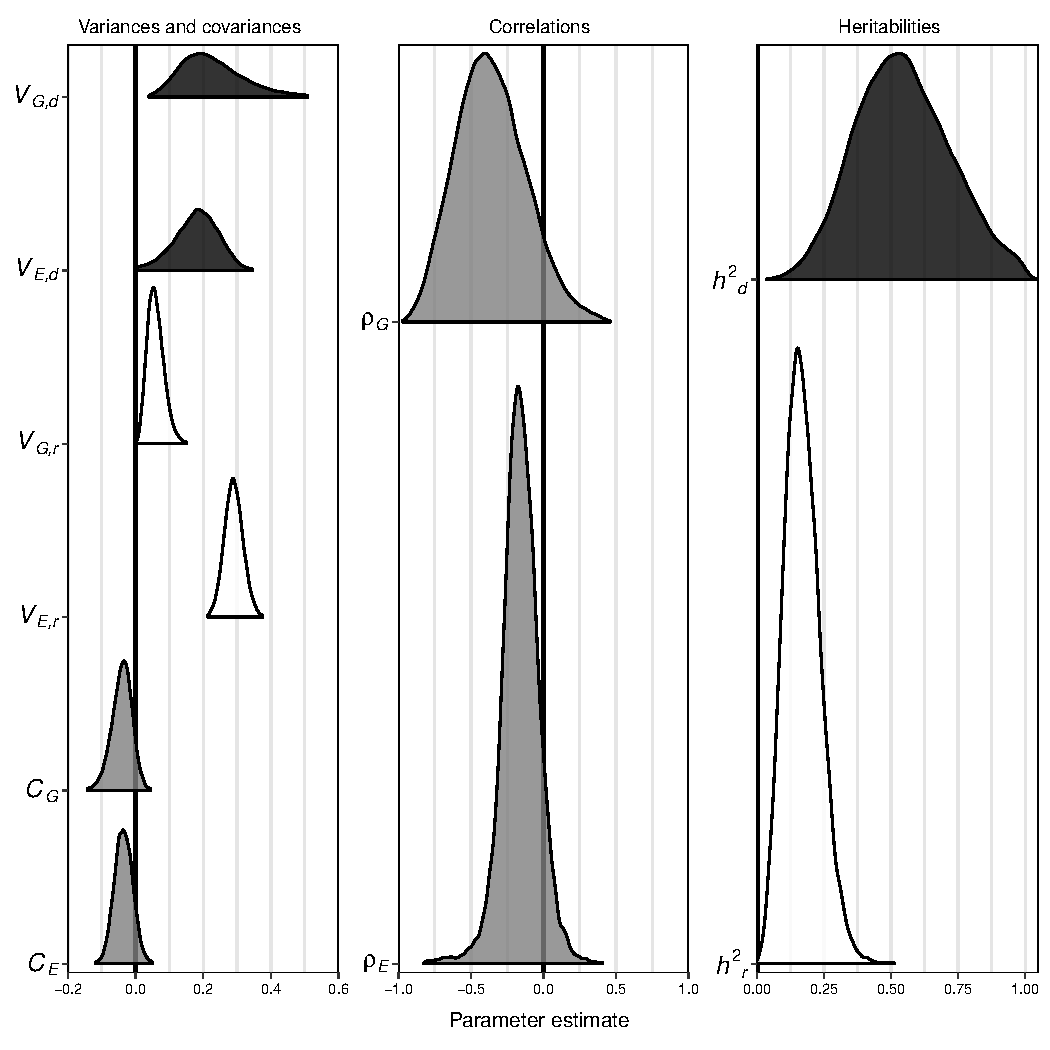
\includegraphics[width=0.75\linewidth]{Figures/corr_posteriors.pdf}
\caption{\textbf{Posteriors of parameter estimates.} Posterior densities of variance- and covariance-related parameter estimates from the animal model. Subscripts identify whether parameters relate to the genetic ($G$) or environmental ($E$) covariance matrices, and whether they describe the dispersal ($d$) or fertility ($r$) trait. Dispersal-related parameters are shown in dark gray, fertility parameters are shown in white, and covariances/correlations between the two traits are shown in light gray. Panels show: trait variances ($V$) and covariances ($C$) (left); trait correlations ($\rho$) (center); and trait heritabilities ($h^{2}$) (right). Note the different x-axis scales.}\label{corr:posteriors}
\end{figure}

\newpage
\subsection*{\textit{Simulation results}}
\subsubsection*{Simulations of \textup{C. maculatus} invasion}
Simulations of eco-ecolutionary spread dynamics using empirical point estimates for genetic and environmental variation in demography and dispersal generated results that were consistent with our previous experimental studies of \textit{C. maculatus} invasions (Figure \ref{corr:barplot}).
After 20 generations, evolving invasions spread farther and had elevated variability in final extent across simulation replicates, compared to invasions with the same amount phenotypic variance but zero trait heritability.
As we found experimentally, the evolutionary effect on variability was proportionally much stronger than the effect on the mean invasion speed.
Trait evolution in the simulated invasions also aligned well with empirical observations: range-edge patches showed a genetically based increase in dispersal ability and virtually no evolved change in fertility (Figure \ref{corr:barplot}).

\begin{figure}[h!]
\centering
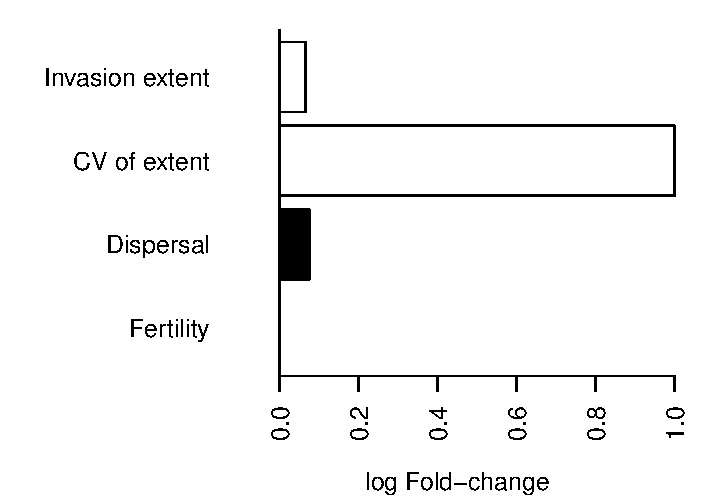
\includegraphics[width=0.5\linewidth]{Figures/foldchange_barplot}
\caption{\textbf{Simulation results for \textit{C. maculatus} invasions.} Bars show the natural logarithm of fold-change due to evolution in invasion metrics and demography and dispersal traits for simulation results corresponding to empirical estimates for \textit{C. maculatus} (Table \ref{corr:estimates}).
White bars show the mean and CV of final extent after 20 generations of spread, and the fold-change is relative to `control' invasions with no genetically based trait variation ($h^{2}_{d} = h^{2}_{r} = 0$).
Black bars show genetically based quantitative trait values for dispersal distance ($\mu^{d} + a^{d}$) and low-density fertility ($\mu^{r} + a^{r}$), and fold-change compares the mean range-edge genotype in generation 20 with the initial genotype in generation 1.}
\label{corr:barplot}
\end{figure}

\subsubsection*{Generalizing beyond the \textup{C. maculatus} system}
\paragraph{Invasion speed and variability}
Beyond the bean beetle-specific parameter estimates, we found that evolutionary changes in invasion speed and variability were general outcomes when there was genetic variation in demography and dispersal traits, but that trait correlations could modify how evolution shapes these ecological measures of spread, quantitatively and even qualitatively.
Simulated invasions were fastest when both genetic and environmental correlations were strongly positive, and slowest when both correlations were strongly negative (Figure \ref{corr:sim_default}A, solid lines).
As expected, genetic correlations only accelerated spread when trait heritabilities were non-zero, while environmental correlations could accelerate spread in the absence of genetic variation (Figure \ref{corr:sim_default}A, dashed lines).
Comparing invasions with and without genetic variation and quantifying their difference in speed as a fold-change (Figure \ref{corr:sim_default}B) shows that evolution accelerated spread even under the strongest negative genetic correlation, where evolved increases dispersal ability necessarily meant evolved decreases fertility, and vice versa.
More positive genetic correlations led to stronger evolutionary acceleration, since selection could favor high-dispersal / high-fertiltiy phenotypes.
Interestingly, the magnitude of evolutionary acceleration responded in the opposite way to environmental correlations, being greatest at negative values.
This was likely because invasions were already accelerated by positive environmental correlations and there was therefore less opportunity for further increases in speed due to trait evolution, given a fixed amount of total phenotypic variation.

Variance in invasion outcome, measured as the CV of final invasion extent across simulation replicates, also responded positively to genetic correlations when trait heritabilities were non-zero (Fig. \ref{corr:sim_default}C,D).
Variance-generating effects of evolution and, consequently, the change in variance with vs. without evolution were both greatest under strong, positive correlations.
However, in contrast to results for the mean speed of invasion, variance across realizations was largely unaffected by environmental correlations.

\begin{figure}[h!]
\centering
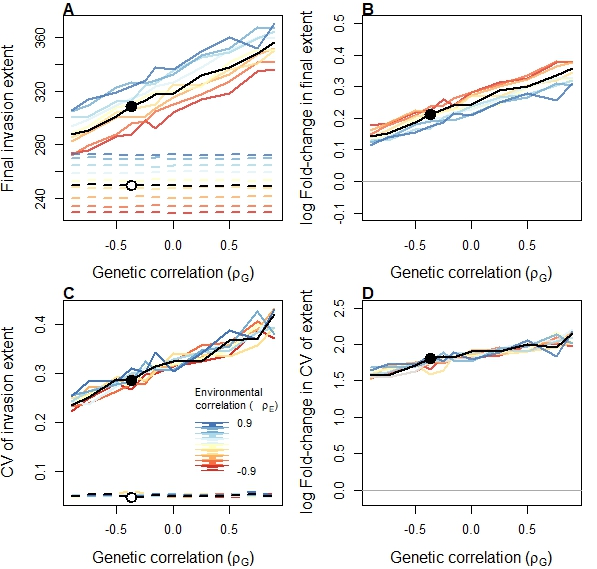
\includegraphics[width=0.75\linewidth]{Figures/sim_invasions_default_h2_4panel}
\caption{\textbf{Simulation results for evolutionary effects on invasion speed and variability.}
\textit{A}, Final invasion extent (patch number); \textit{B}, Fold-change in final extent due to evolution; \textit{C}, Coefficient of variation (CV) of invasion extent; \textit{D}, Fold-change in CV due to evolution.
For all panels, responses are shown in relation to $\rho_{G}$ (\textit{x}-axes) and $\rho_{E}$ (colored lines).
In \textit{A},\textit{C} dashed and solid lines show simulation output for zero and non-zero trait heritabilities, respectively, where non-zero values correpond to \textit{C. maculatus} (Table \ref{corr:estimates}); panels \textit{B},\textit{D} contrast these cases as fold-change.
Black lines show results for the $\rho_{E} = -0.16$ and points further show $\rho_{G} = -0.37$, the point estimates from the \textit{C. maculatus} system.}
\label{corr:sim_default}
\end{figure}

Figure \ref{corr:sim_default} shows the influence of trait correlations for point values of trait heritabilities and variances estimated from the beetle system, where black lines and points identify the beetle system in the context of variation in $\rho_{G}$ and $\rho_{E}$.
This visualization illustrates how empirically observed increases in invasion speed and variability due to evolution were likely constrained by the negative genetic correlation between dispersal and fertility, while the negative environmental correlation enhanced the evolutionary effect on mean speed.
As shown in Online Appendix B, we found qualitatively identical results for evolutionary effects on invasions when we varied parameters of trait architecture ($h^{2}_d$, $h^{2}_r$, $V_{P,d}$, $V_{P,r}$), with one important exception: with more phenotypic variation and higher trait (especially fertility) heritability than we observed in the beetle system, it was possible for evolution to \textit{decelerate} invasion (Fig. \ref{corr:sim_vary_h2_Pvar}).
The evolutionary decrease in invasion speed occurred only when genetic correlations were very negative, where the best dispersers at the leading edge were very likely to carry low-fertility genotypes.
Even under conditions where evolution decelerated spread, evolutionary effects on variance remained positive.
Thus, the evolutionary increase in variance across realizations of spread was a general result across the dimensions of parameter space that we considered, but the evolutionary increase in average speed was not.

\paragraph{Trait evolution}
Simulation results for evolved trait changes provide a mechanistic basis for the invasion metrics described above, and help contextualize the trait changes observed in the \textit{C. maculatus} system (Fig. \ref{corr:traits}).
Dipsersal showed strong, positive evolutionary responses across all values of genetic and environmental correlations.
In contrast, evolutionary change in fertility during invasion was strongly dependent on the sign and magnitude of genetic correlations.
Under no correlation ($\rho_{G}$ = 0), there was a small evolved increase in fertility, consistent with theoretical expectations for `\textit{r}-selection’ on fertility at low-density wave fronts.
However, strong evolved increases in fertility occurred only when it was positively genetically linked to dispersal.
On the other hand, negative correlations caused either no change or an evolved decrease in fertility at the invasion front, depending on the magnitude of the correlation.
%Thus, our previous finding of no evolved changed in fertility during \textit{C. maculatus} range expansion was at least partially driven by its negative genetic correlation with dispersal.

Regardless of direction, the magnitude of the evolutionary response in fertility was lower than that of dispersal (Fig. \ref{corr:traits}).
This was true for the trait architecture correspding to \textit{C. maculatus}, where there was more additive genetic variance in dispersal than in fertility (Fig. \ref{corr:posteriors}).
However, that asymmetry alone does not explain the stronger evolutionary response of dispersal.
In Online Appendix C, we show that spatial selection on dispersal generally predominated `\textit{r}-selection’ on low-density fertility, even when fertility was as or more heritable than dispersal distance (cite figure).
Across the entire parameter space we considered, strong, positive evolutionary responses in fertility occurred only when it was positively genetically linked with dispersal, but not \textit{vice versa}. 
Finally, also in Online Appendix C, we show that variability in range-edge trait values across simulation replicates was generally greatest for both traits under positive correlations, consistent with the increase in variability of invasion outcomes under positive correlations (Fig. \ref{corr:sim_default}C,D). \footnote{\tom{I still need to make this figure.}}

\begin{figure}[h!]
\centering
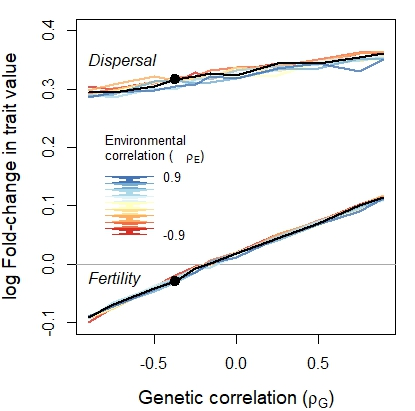
\includegraphics[width=0.5\linewidth]{Figures/trait_change}
\caption{\textbf{Simulation results for evolutionary change in dispersal and fertility.} Lines show the natural logarithm of fold-change in dispersal (log(patches)) and fertility (log(offspring)) in relation to $\rho_{G}$ (\textit{x}-axis) and $\rho_{E}$ (colored lines). 
Fold-change compares trait values ($\mu^{d} + a^{d}$ and $\mu^{r} + a^{r}$) in the farthest occupied patch after 20 generations of range expansion to their respective starting values. 
Black lines show results for the $\rho_{E} = -0.16$ and point shows $\rho_{G} = -0.37$, the point estimates from the \textit{C. maculatus} system.}
\label{corr:traits}
\end{figure}

% Discussion -------------
\section*{Discussion}
Long-standing ecological theory and more recent eco-evolutionary work emphasize the key roles of demography and dispersal traits, and the evolutionary forces that act on them, as drivers of invasion dynamics. But, in both classes of theory, regeneration and movement are usually assumed to operate independently.
On the other hand, different bodies of literature emphasize connections between demography and dispersal traits through a myriad of mechanisms, ranging from trade-offs and costs of dispersal (typically corresponding to negative corrrelations) to dispersal `syndromes' that package several life history and movement traits into a multivariate phenotype (typically corresponding to positive correlations).
Our work unifies both ends of this continuum into a cohesive framework for understanding the role of trait correlations in invasion dynamics, and carries significance at two levels.
First, the quantitative genetics experiment and empirically parameterized simulation model allowed us to retrospectively diagnose the contributions of demography-dispersal correlations to observed spread dynamics and trait evolution in the \textit{C. maculatus} model system.
Our findings that trait architecture, including genetic and environmental variances and covariance, imposed important constraints on trait evolution and invasion dynamics provide a novel window of insight onto this empirical case study. 
Second, the generalized simulation model expanded our breadth of inference, revealing which outcomes were particular to the trait architecture of \textit{C. maculatus} and which were more general.
Collectively, our results identify trait correlations as a key factor modulating how evolution shapes trajectories of biological invasion.

Simulated invasions based on \textit{C. maculatus} parameters recapitulated our previous experimental results \citep{ochocki_rapid_2017}: invasions subject to the influence of selection on dispersal and fertility at the low-density leading edge were faster, on average, and more variable, and showed evolved increases in dispersal but not fertility, compared to invasions in which that influence was suppressed (Figure \ref{corr:barplot}).
This correspondence bolstered our confidence that the simulation model was an appropriate vehicle for testing how trait correlations contributed to those results.
We found that evolutionary increases mean and variance were expected for \textit{C. maculatus} regardless of trait correlations -- even a strict genetic trade-off ($\rho_{G} = -1$) could not have prevented evolutionary acceleration -- but the sign and magnitude of correlations could modify the strength of the response.
Specifically, increasing the genetic correlation from negative to positive values increased the speed of invasion, on average, as well as its variability across realizations.
Thus, the negative genetic correlation that we detected between dispersal and fertility in \textit{C. maculatus} (Fig. \ref{corr:posteriors}) caused the evolutionary increases in invasion speed and variability observed in our prevoius study to be weaker than they would have been under no, or especially positive, genetic correlations (Fig. \ref{corr:sim_default}).

The increase in invasion speed with increasing strength of demography-dispersal correlation was a general result, not limited to beetle-specific parameter estimates (Fig \ref{corr:sim_vary_h2_Pvar}).
This likely occurred because positive correlations align the dominant axis of phenotypic variation with the direction of selection, with high-dispersal / high-fertility (and therefore high-invasion speed) phenotypes favored at the leading edge \citep{phillips_life-history_2010}.
The accelerating effect of positive genetic correlations may also reflect some contribution of `enhanced spatial selection', whereby greater reproductive rates at the leading edge strengthen spatial selection on dispersal \citep{perkins_evolution_2013}.
On the other hand, negative genetic correlations constrain evolutionary acceleration of invasion, since an evolved increase in one trait would mean an evolved decrease in the other.
Importantly, our simulations revealed that a strongly negative demography-dispersal genetic correlation, combined with a large amounts of heritable variation, can actually \textit{decelerate} invasion, a new result as far as we are aware.
It is unknown how commonly conditions align to cause evolutionary deceleration of expanding populations, but the possibility of it should cause us to reconsider general expectations for eco-evolutionary invasion dynamics in light of genetic architecture.

In addition to increasing the average speed of invasion, evolution of demography and dispersal traits can also amplify variability across realizations of spread.
This result that has been shown in previous theoretical and experimental studies (\citealt{ochocki_rapid_2017}; \citealt{weiss-lehman_rapid_2017}; \citealt{phillips_evolutionary_2015}; but see \citealt{williams_rapid_2016}) and is typically interpreted as a signature of `gene surfing', whereby founder events at the low-density leading edge lead to stochastic allele fixation, either reinforcing or counter-acting selection on demography and dispersal \citep{edmonds_mutations_2004,klopfstein_fate_2006,excoffier_surfing_2008,peischl_expansion_2015}.
Our new results indicate that genetic correlations are an important modifier of invasion variability (Fig. \ref{corr:sim_default}), likely for reasons related to their influence on average speed.
Under a positive genetic correlation, the major axis of phenotypic variance spans low-dispersal / low-fertility (and thus low invasion speed) to high-dispersal / high-fertility (and thus high invasion speed).
Stochastic fixation of alleles sampled from this axis of variation should therefore generate a wide range of invasion speeds across realizations.
Conversely, under a negative genetic correlation, the major axis of phenotypic variance spans low-dispersal / high-fertility to \textit{vice versa}; opposite ends of this axis are phenotypically different but similar in their resulting invasion speeds, due to the counter-acting effects of the two traits.
The corresponding range of variation in invasion speed should therefore be smaller than under a positive correlation, all else equal.
In this way, increasing a genetic correlation between demography and dispersal from negative to positive values increases the opportunity for fixation of ecologically different phenotypes.
Empirical work has shown that evolutionary effects on replicate-to-replicate invasion variance may themselves be highly variable across systems \citep{ochocki_rapid_2017,weiss-lehman_rapid_2017,williams_rapid_2016,van2018kin}.
Our results suggest that, as with mean invasion speed, understanding the genetic architecture of demography and dispersal traits may help resolve this heterogeneity across studies.

In addition to the large-scale patterns of mean and variance in invasion speed, our results also provide insight into underlying mechanisms: trait evolution during range expansion.
Empirical studies of range-core vs. range-edge values for life history and movement traits have been rapidly accumlating, often but not always supporting the theoretical expectation of increased dispersal and reproductive output at the range edge (reviewed in \citealt{chuang_expanding_2016}).
Our results show that, in the \textit{C. maculatus} system (Fig. \ref{corr:traits}) and in general, the evolutionary response of dispersal ability exceeded that of low-density reproductive rate, which only showed a strong evolved increase when it was genetically linked to dispersal ability.
Furthermore, under negative genetic correlations, it was always dispersal that increased at the expense of fertility (evolutionary acceleration occurred as long as gains in dispersal more than compensated for losses in fertility).
These results point to two reasons why we failed to detect any evolved change in fertility in our previous invasion experiment: the pre-dominance of spatial selection on dispersal over \textit{r}-selection on fertility, and the negative genetic correlation between the two, which further limited any evolved increase.
Our trait evolution results also shed light on empirical results elsewhere in the literature, including evidence for evolved increases in dispersal but decreases in fertility in range-edge populations \citep{simmons_changes_2004,hughes_evolutionary_2003}.
Working with laboratory invasions of flour beetles, \cite{weiss-lehman_rapid_2017} found that evolution increased the mean and variance of invasion speed at the population-level, while at the trait level dispersal increased but fertility significantly decreased; in our simulations, a negative genetic correlation often yielded exactly these results. 
By considering both invasion dynamics and underlying traits, our results highlight their sometimes counter-intuitive connections, including cases where evolved increases in dispersal ability may fail to accelerate or even decelerate range expansion due to corresponding reductions in fertility.

While genetic correlations are clearly consequential for the eco-evolutionary dynamics of spread, our work also provides guidance on the relative roles of genetic vs. environmental trait correlations, both of which are commonly reported in the literature and were detected in the \textit{C. maculatus} system (Fig. \ref{corr:posteriors}).
Positive phenotypic correlations that cause high-dispersal / high-fertility trait values to co-occur within individuals at the expanding front will always have a positive effect on the speed of invasion, and \textit{vice versa} for negative phenotypic correlations, regardless of whether or not the trait correlation is genetically based.
Thus, in regard to effects on invasion speed, genetic and environmental correlations were qualitatively interchangeable (Fig. \ref{corr:sim_default}).
However, in invasion variability and trait evolution, the roles of genetic correlations were generally much greater than those of environmental correlations.
Thus, as future studies begin to consider demography-dispersal correlations in spread dynamics, there may be some contexts or applications in which isolating genetic vs. environmental contributions would be of little importance, and others where separating the two may be critical. 

There are some assumptions and limitations of our work that merit consideration and that may suggest avenues for future research.
First, while we explore environmental sources of trait variation, the environments of both our empirical system and simulation model were constant and homogeneous. 
It is like that we would have detected a stronger signal of non-genetic variation in our empirical estimates, and  a stronger influence of environmentally-based trait correlations in our simulations, with a more realistic, heterogeneous landscape. 
Second, we have treated trait correlations as statistical phenomena; we know little about how or why they arise in the beetle system, biologically.
Similarly, the two traits that we consider are more likely `meta-traits' that capture many physiological and behavioral processes.
Understanding these lower-level mechanisms was not essential for the purposes of our study, but may be important in other contexts. 
Third, our quantitative genetics model was relatively simple, including only additive genetic and environmental components. 
Other, potentially important sources of trait variation include maternal, dominance, epistatic, and epigenetic effects, all of which would have been rolled into our additive genetic estimates due to their association with kinship.
It is common for models of quantitative traits to focus exclusively on additive genetic and environmental effects, as we have done \citep{wilson_ecologists_2010}, but it would be useful to know, in our empirical system and generally, how much bias is introduced by this simplifying assumption, and how it could affect key conclusions. 

\paragraph*{Conclusion}
In summary, our work provides a new level of understanding for how rapid evolution of demography and dispersal traits can modify the dynamics of biological invasion.
That trait architecture matters should surprise no one; yet, until now, there has been little guidance on how it matters. 
We show that trait correlations are an important modifier on the eco-evolutionary dynamics of spread, able to amplify or constrain -- in some cases, reverse -- evolutionary increases in invasion speed and variability. 
Our findings should aid in the interpretation of empirical patterns of trait evolution and population expansion, as we have shown with our bean beetle case study. 
As studies of individual heterogeneity increasingly intersect with classic ecological questions and models, the ways in which trait values may co-vary across individuals will be an important consideration, as our work demonstrates. 

\section*{Acknowledgements}
Funding for this work was provided by NSF-DEB-1501814 and by NSF Data Analysis and Visualization Cyberinfrastructure grant OCI-0959097, which supports computing facilities at Rice University. We thank M. Zapata for help in conducting the experiment. We also thank A. Bibian, A. Compagnoni, C. Dytham, K.B. Ensor, L. Lancaster, V.H.W. Rudolf, E. Schultz, E. Siemann, M. Sneck, J.M.J. Travis, and M.E. Wolak for comments on the project and manuscript.

\newpage{}
\section*{Online Appendix A: Additional Simulation Methods}
Each generation of the simulation, individuals in the population mated, reproduced, died, and their offspring dispersed; this is similar to the laboratory-imposed life-cycle in \textit{C. maculatus} invasion experiments \citep{miller_sex_2013,wagner_genetic_2016,ochocki_rapid_2017}.
Because the landscape was modeled as an array of discrete patches, local interactions -- including mate finding, reproduction, and density-dependent population growth -- took place at the patch-level.
%Thus, the population density in any patch was simply the total number of individuals in that patch.
For mating, each individual selected one other individual in the same patch, at random (and with replacement), and received genetic information from that individual.
Because individuals were modeled as hermaphrodites, all individuals were capable of acting as both male and female during reproduction.
Under this mating system, each individual had the capacity to contribute genetic information to multiple unique individuals, but could only receive genetic information from one individual.
Individuals could not self-fertilize; all offspring were thus the product of two unique parents.
In instances where a patch contained only one individual, that individual did not reproduce.
Our model therefore includes a mate-finding Allee effect for singly-occupied patches.

Offspring inherited breeding values from their parents $\bm{a}_{jk}$ , which were drawn from a multivariate normal distribution according to Equation (\ref{corr:gen}).
The expressed phenotype was also dependent on the environmental deviates $\bm{e}_{i}$, drawn according to Equation (\ref{corr:env}), and the population mean phenotypes $\mu^{d}$ and $\mu^{r}$.
As in similarly structured models of evolution during invasions, additive genetic variance is expected to decrease as the variance in breeding values among individuals decreases \citep{phillips_evolutionary_2015}.
Each generation, we calculated the additive genetic covariance matrix $\bm{G}$ in each patch by calculating the variances and covariance among all breeding values in that patch.
Offspring breeding values were then assigned according to Equation (\ref{corr:gen}), using the patch-estimated $\bm{G}$ matrix.

After mating, each individual reproduced following the density-dependent Beverton-Holt model of population growth described in Equations (\ref{corr:BevHoltFull}) to (\ref{corr:BevHoltPercap}).
We modeled invasions across a homogeneous landscape, assuming a fixed resource density of 10 beans in all patches. The carrying capacity $K$ was therefore fixed across the landscape, but per-capita population growth varied among individuals according to \ref{corr:fert_linmod}.

After reproduction, parents senesced, marking the end of the generation; at the start of the next generation, their offspring dispersed.
Thus, we modeled populations that were characterized by discrete, non-overlaping generations.
Offspring dispersed from their natal patch according to their latent dispersal phenotype $\lambda_{ijk}$, and dispersal distance was Poisson distributed, as in Equation (\ref{corr:dispersal}).
While the Poisson distribution only generates positive values, individuals in the simulation could disperse either to the left or right. We simulated bi-directional dispersal by randomly multiplying an individual's Poisson distance by -1 (for leftward dispersal) or +1 (for rightward dispersal), with equal probability for each direction.
After dispersal, individuals mated with an individual in the patch that they dispersed to, they reproduced, and they senesced.
We simulated this process for 20 generations, on par with similar timescales of eco-evolutionary dynamics in empirical systems \citep{williams_rapid_2016,ochocki_rapid_2017,weiss-lehman_rapid_2017}.

Parameter values and definitions are provided in Table \ref{corr:params}. In addition to varying the genetic and environmental trait correlations, as described in the main text, we also explored five cases corresponding to variation in heritability of dispersal and fertility:
\begin{itemize}
  \item $h^{2}_d = h^{2}_r = 0$. The `no evolution' scenario, which serves as an internal control and a baseline for quantifying evolutionary effects.
  \item $h^{2}_d > h^{2}_r$. Heritability of dispersal greater than that of fertility (matching the beetle system: Results).
  \item $h^{2}_d < h^{2}_r$. Heritability of fertility is greater than that of dispersal (opposite of the beetle system).
  \item $h^{2}_d = h^{2}_r$. Equally high heritability of dispersal and fertility (equalling the higher heritability from the beetle system).
  \item $h^{2}_d = h^{2}_r$. Equally low heritability of dispersal and fertility (equalling the lower heritability from the beetle system).
\end{itemize}
Lastly, we repeated all of the above for two levels of total phenotypic variance: $V_{P,d}$ and $V_{P,r}$ from the beetle system and $2V_{P,d}$ and $2V_{P,r}$.
This allowed us to assess whether changing heritabilities (proportions of variance) has qualitatively consistent effects for different absolute amounts of variance.

All simulations were conducted using Julia 0.5.0 \citep{bezanson_julia:_2017}, and all analyses were conducted using R 3.4.0 \citep{r_core_team_r:_2015}.
All code for the simulation and analyses is publicly available at \url{https://github.com/bochocki/correlatedtraits}.

\renewcommand{\thetable}{A\arabic{table}}
\setcounter{table}{0}
\begin{table}[h]
\centering
\label{Parameter values and definitions}
\caption[Parameter values and definitions]{\textbf{Parameter values and definitions.} Descriptions of key parameters in the simulation.}\label{corr:params}\vspace{0.1in}
\begin{tabularx}{0.95\linewidth}{llX}
\toprule
Parameter    & Value(s)                               & Definition                                        \\ \midrule
$N_{0}$      & 20                                     & Initial population size                           \\
$\mu_{d}$    & 1.63                                   & Initial mean dispersal phenotype   \\
$\mu_{r}$    & 2.74                                   & Initial mean fertility phenotype
\\
$V_{P,d}$    & [0.4, 0.8]                                   & Initial total phenotypic variance in dispersal \\
$V_{P,r}$    & [0.35, 0.7]                                   & Initial total phenotypic variance in fertility \\
$h^{2}_{d}$  & [0.0, 0.17, 0.54]                                   & Heritability of dispersal                  \\
$h^{2}_{r}$  & [0.0, 0.17, 0.54]                                   & Heritability of fertility                \\
$\rho_{G}$   & [-0.9, -0.5, -0.37, -0.16, -0.1,       & Additive genetic correlation          \\
             & \phantom{$[-$}0.0, 0.1, 0.5, 0.9]      &                                                   \\
$\rho_{E}$   & [-0.9, -0.5, -0.37, -0.16, -0.1,       & Environmental correlation             \\
             & \phantom{$[-$}0.0, 0.1, 0.5, 0.9]      &                                                   \\
$K$          & 3.81                                   & Carrying capacity per bean                          \\
Generations  & 20                                     & Number of generations of invasion                 \\
Replicates   & 1000                                   & Number of simulation replicates                   \\ \bottomrule
\end{tabularx}
\end{table}

\newpage{}
\section*{Online Appendix B: Additional Simulation Results}
\renewcommand{\thefigure}{B\arabic{figure}}\setcounter{figure}{0}
\setcounter{figure}{0}

\begin{figure}[h!]
\centering
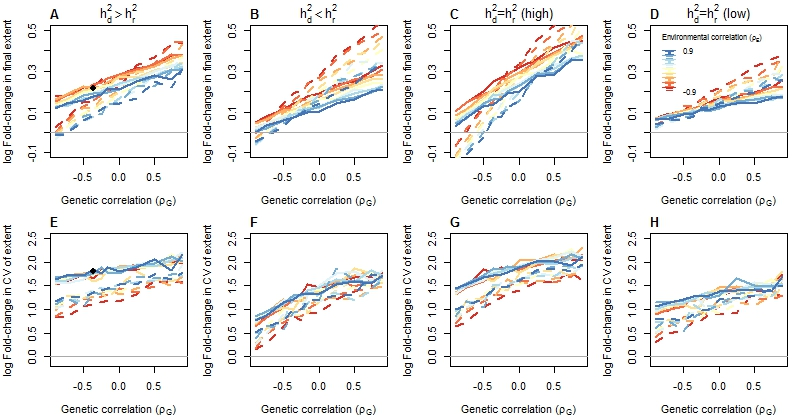
\includegraphics[width=1\linewidth]{Figures/sim_invasions_vary_h2_vary_Pvar}
\caption{\textbf{Expanded parameter space for invasion mean and variance.}
Lines show the natural logarithm of fold-change in mean invasion extent (\textit{A}-\textit{D}) and CV of invasion extent (E-F) in relation to $\rho_{G}$ (\textit{x}-axis) and $\rho_{E}$ (colored lines). Columns correspond to alternative scenarios of dispersal and fertility heritabilities. \textit{A} and \textit{E} correspond to empirical estimates from \textit{C. maculatus}; \textit{B} and \textit{F} correspond to \textit{C. maculatus} heritabilities swapped between traits; \textit{C} and \textit{G} show equal heritabilities set to the higher of the two; \textit{D} and \textit{H} show equal heritabilities set to the lower of the two. 
Line types show the total phenotypic variances estimated from the beetle system (solid), or twice the variances from the beetle system (dashed).
Black point corresponds to $\rho_{E} = -0.16$ and $\rho_{G} = -0.37$, the point estimates from the \textit{C. maculatus} system.}
\label{corr:sim_vary_h2_Pvar}
\end{figure}

\newpage{}

\begin{figure}[h!]
\centering
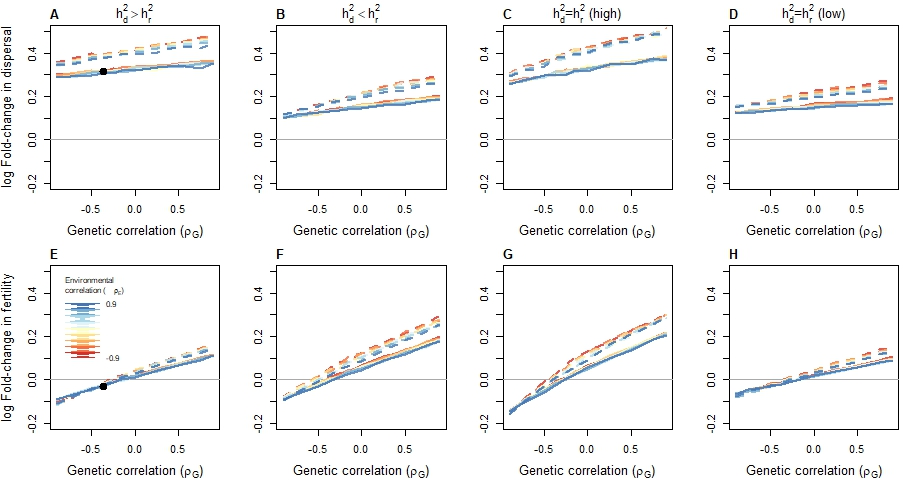
\includegraphics[width=1\linewidth]{Figures/trait_change_appendix}
\caption{\textbf{Expanded parameter space for evolutionary change in dispersal and fertility.} Lines show the natural logarithm of fold-change in dispersal (log(patches)) and fertility (log(offspring)) in relation to $\rho_{G}$ (\textit{x}-axis) and $\rho_{E}$ (colored lines). 
Fold-change compares trait values ($\mu^{d} + a^{d}$ and $\mu^{r} + a^{r}$) in the farthest occupied patch after 20 generations of range expansion to starting values. 
Black point corresponds to $\rho_{E} = -0.16$ and $\rho_{G} = -0.37$, the point estimates from the \textit{C. maculatus} system.
Columnes and line types as in Fig. \ref{corr:sim_vary_h2_Pvar}.}
\label{corr:traits_app}
\end{figure}

%%%%%%%%%%%%%%%%%%%%%
% Bibliography
%%%%%%%%%%%%%%%%%%%%%
\newpage{}
\bibliographystyle{references/amnat}
\bibliography{references/biblio}


%%%%%%%%%%%%%%%%%%%%%
% Tables
%%%%%%%%%%%%%%%%%%%%%
%\section*{Tables}

\end{document}
